\documentclass[12pt]{article}
\usepackage{fancyhdr}
\usepackage{amsmath}
\usepackage{amsthm}
\usepackage{mathtools}    
\usepackage{enumitem}
\usepackage[Export]{adjustbox}
\usepackage{cancel}
\usepackage{algorithm}
\usepackage[noend]{algpseudocode}
\usepackage{graphicx}
\usepackage[margin = 1in]{geometry}
\usepackage{blindtext}
\usepackage[section]{placeins}
\usepackage{xcolor,listings}
\usepackage{textcomp}
\lstset{upquote=true}

\pagestyle{fancy}
\fancyhead{}
\fancyfoot{}
\usepackage[T1]{fontenc}
\fancyhead[L]{Proiect SGBD}
\fancyhead[R]{Student Țânțaru Dragoș-Constantin, grupa 244}
\setlength{\headheight}{18pt}
\fancyfoot[C]{\thepage}
\title{Bază de date pentru gestionarea unei afaceri cu librării}
\author{Dragoș-Constantin Țânțaru}

\begin{document}
\maketitle
\thispagestyle{fancy} 
\section{Cerința 1. Descrierea proiectului}
Am construit o bază de date care are ca scop facilitarea conducerii unei afaceri de tip librărie. Este posibil ca afacerea să aiba mai multe librării în posesia sa. De asemenea, am considerat că un angajat poate lucra la mai mult de o singura librărie, ca exemplu ar fi un manager ce se ocupă de mai multe librării sau un IT-ist care administrează sistemele informatice de la diferite librării.\\
Am implementat si funcționalitatea bazei de date de a admite „membrii” ai afacerii. Un membru este un client ce a achiziționat un tip de abonament. Abonamentele reprezinta o plata lunară făcută de client, in schimbul căreia are acces la o mulțime de cărți în format digital.\\
Baza de date asigură toate aceste utilități și multe altele. Fără o bază de date, ar fi dificil pentru o afacere să poată menține o evidență corectă, nemaivorbind de diversele aplicații care se pot implementa facil cu o bază de date, dar care ar fi greu de realizat altfel.
\section{Diagrama Entitate-Relație}
\begin{figure}[!htb]
	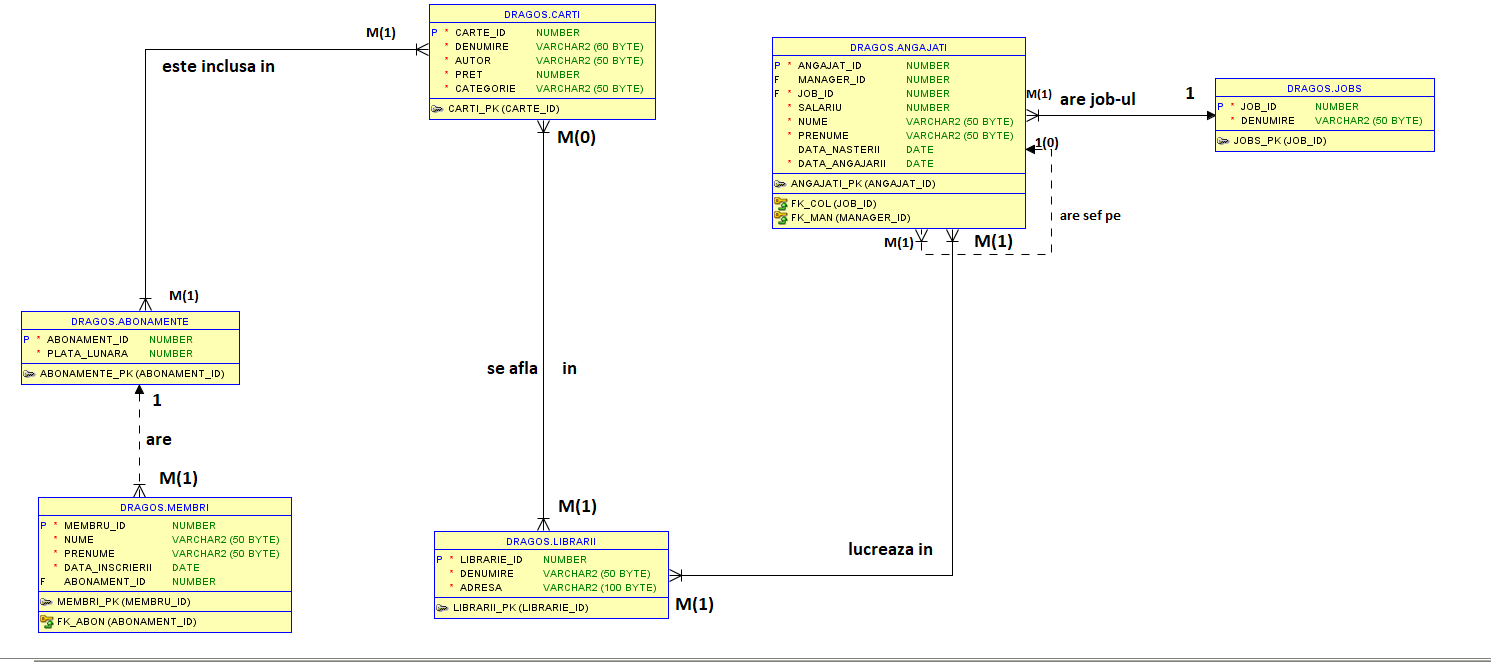
\includegraphics[max width=\linewidth]{imgs/diagER.png}
	\caption{diagrama ER}
	\label{fig:ER}
\end{figure}
\section{Diagrama Conceptuala}
\begin{figure}[!htb]
	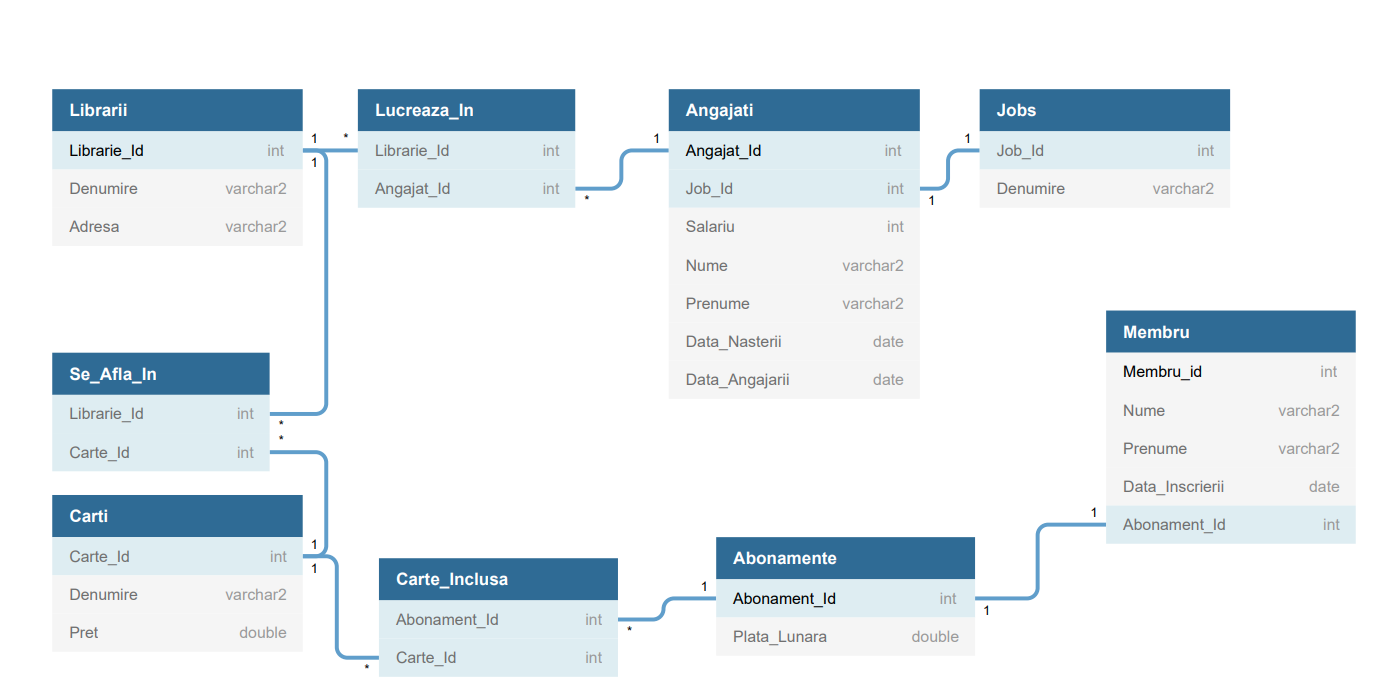
\includegraphics[max width=\linewidth]{imgs/diagConceptuala.png}
	\caption{diagrama Conceptuala}
	\label{fig:Conceptuala}
\end{figure}
\section{Definirea tabelelor}
\begin{lstlisting}[language=SQL,
				  showspaces=false,
				  basicstyle=\ttfamily,
				  numbers=left,
				  numberstyle=\tiny,
				  commentstyle=\color{gray}]
CREATE TABLE Librarii (
Librarie_Id NUMBER NOT NULL,
Denumire VARCHAR2(50) NOT NULL,
Adresa VARCHAR2(100) NOT NULL,
PRIMARY KEY (Librarie_Id)
);

CREATE TABLE Carti (
Carte_Id NUMBER NOT NULL,
Denumire VARCHAR2(60) NOT NULL,
Autor VARCHAR(50) NOT NULL,
Pret NUMBER NOT NULL,
Categorie VARCHAR2(50) NOT NULL,
PRIMARY KEY (Carte_Id)
);

CREATE TABLE Abonamente(
Abonament_Id NUMBER NOT NULL,
Plata_Lunara NUMBER NOT NULL,
PRIMARY KEY (Abonament_Id)
);

CREATE TABLE Membri (
Membru_Id NUMBER NOT NULL,
Nume VARCHAR2(50) NOT NULL,
Prenume VARCHAR2(50) NOT NULL,
Data_Inscrierii DATE NOT NULL,
Abonament_Id NUMBER,
PRIMARY KEY (Membru_Id),
CONSTRAINT fk_abon
FOREIGN KEY (Abonament_Id)
REFERENCES Abonamente(Abonament_Id)
);

CREATE TABLE Carte_Inclusa(
Abonament_Id NUMBER NOT NULL,
Carte_Id NUMBER NOT NULL,
PRIMARY KEY (Abonament_Id, Carte_Id),
CONSTRAINT fk_col_ab
FOREIGN KEY (Abonament_Id)
REFERENCES Abonamente(Abonament_Id),
CONSTRAINT fk_col_car
FOREIGN KEY (Carte_Id)
REFERENCES Carti(Carte_Id)
);

CREATE TABLE Se_Afla_In (
Librarie_Id NUMBER NOT NULL,
Carte_Id NUMBER NOT NULL,
PRIMARY KEY (Librarie_Id, Carte_Id),
CONSTRAINT fk_asoc_sb
FOREIGN KEY (Librarie_Id)
REFERENCES Librarii(Librarie_Id),
CONSTRAINT fk_asoc_sc
FOREIGN KEY (Carte_Id)
REFERENCES Carti(Carte_Id)
);


CREATE TABLE Jobs (
Job_Id NUMBER NOT NULL,
Denumire VARCHAR2(50) NOT NULL,
PRIMARY KEY (Job_Id)
);

CREATE TABLE Angajati (
Angajat_Id NUMBER NOT NULL,
Manager_Id NUMBER DEFAULT NULL,
Job_Id NUMBER NOT NULL,
Salariu NUMBER NOT NULL,
Nume VARCHAR2(50) NOT NULL,
Prenume VARCHAR2(50) NOT NULL,
Data_Nasterii DATE DEFAULT NULL,
Data_Angajarii DATE NOT NULL,
PRIMARY KEY (Angajat_Id),
CONSTRAINT fk_col
FOREIGN KEY (Job_Id)
REFERENCES Jobs(Job_Id),
CONSTRAINT fk_man
FOREIGN KEY (Manager_Id)
REFERENCES Angajati(Angajat_Id)
);

CREATE TABLE Lucreaza_In (
Librarie_Id NUMBER NOT NULL,
Angajat_Id NUMBER NOT NULL,
PRIMARY KEY(Librarie_Id, Angajat_Id),
CONSTRAINT fk_asoc_b
FOREIGN KEY (Librarie_Id)
REFERENCES Librarii(Librarie_Id),
CONSTRAINT fk_asoc_a
FOREIGN KEY (Angajat_Id)
REFERENCES Angajati(Angajat_Id)
);
\end{lstlisting}
\begin{figure}[!htb]
	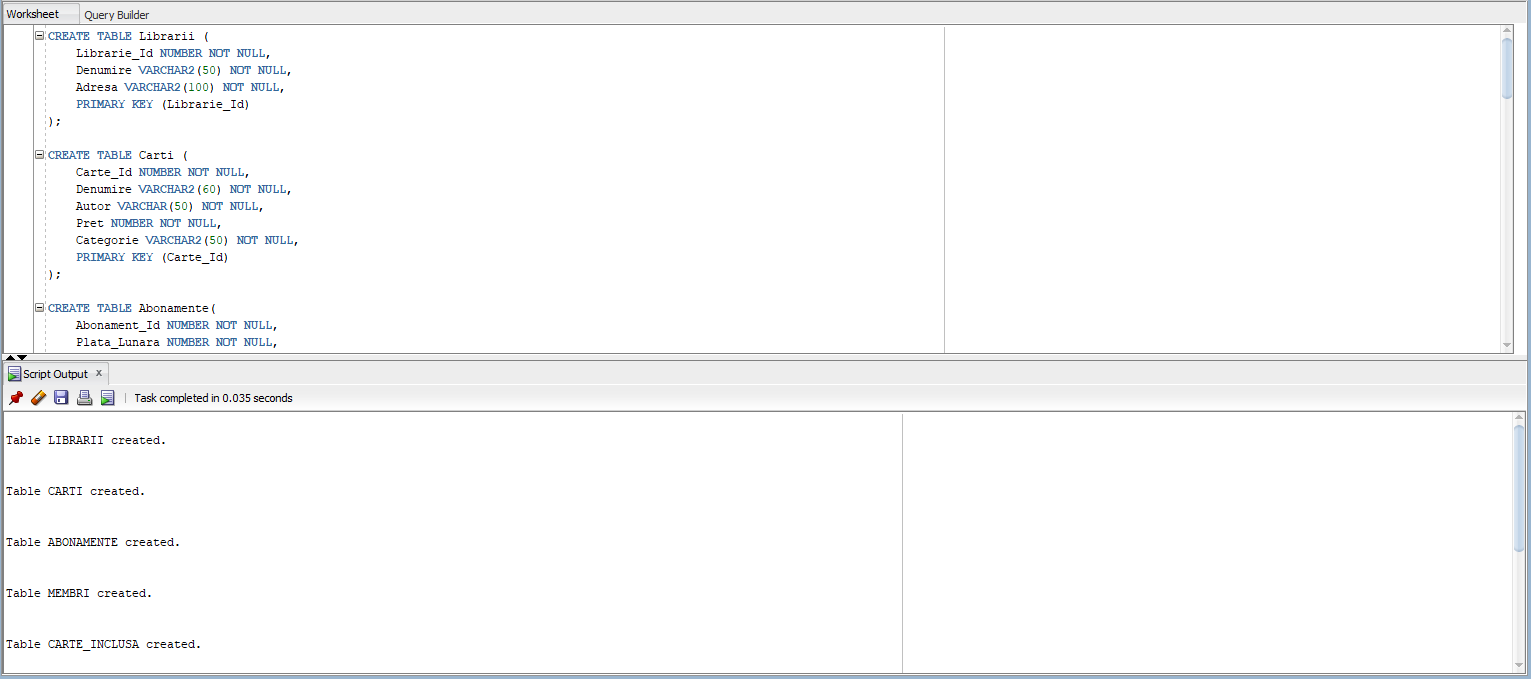
\includegraphics[max width=\linewidth]{imgs/creates1.png}
	\caption{creates 1}
	\label{fig:creates 1}
\end{figure}
\begin{figure}[!htb]
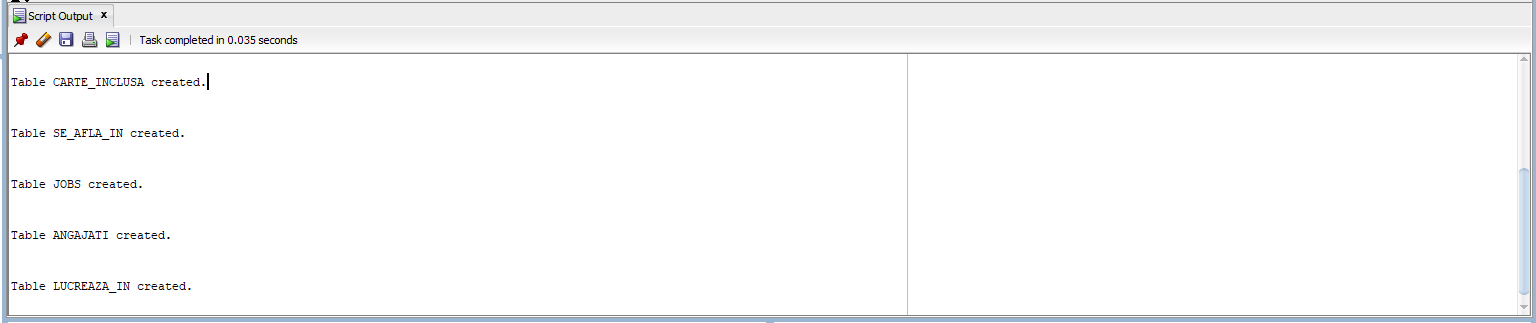
\includegraphics[max width=\linewidth]{imgs/creates2.png}
\caption{creates 2}
\label{fig:creates 2}
\end{figure}
\section{Inserări in tabel}
\begin{lstlisting}[language=SQL,
	showspaces=false,
	basicstyle=\ttfamily,
	numbers=left,
	numberstyle=\tiny,
	breaklines=true,
	commentstyle=\color{gray}]
INSERT INTO Librarii
VALUES (1, 'Libraria abc', 'Strada Unirii nr. 23');
INSERT INTO Librarii
VALUES (2, 'Mihai Eminescu', 'Strada Octavian Goga nr. 26');
INSERT INTO Librarii
VALUES (3, 'Libraria veche', 'Bulevardul Mare nr. 1');

INSERT INTO Jobs
VALUES(1, 'Manager'); 
INSERT INTO Jobs
VALUES(2, 'Librar');
INSERT INTO Jobs
VALUES(3, 'IT-ist');
INSERT INTO Jobs
VALUES(4, 'Contabil');

INSERT INTO Angajati
VALUES(1, NULL, 1, 10000, 'Sefescu', 'Ion', TO_DATE('1972-10-11', 'YYYY-MM-DD'), TO_DATE('1996-07-23', 'YYYY-MM-DD'));
INSERT INTO Angajati
VALUES(2, 1, 2, 3000, 'Pop', 'Andrei', TO_DATE('1975-07-02', 'YYYY-MM-DD'), TO_DATE('1998-02-03', 'YYYY-MM-DD'));
INSERT INTO Angajati
VALUES(3, 1, 2, 3000, 'Bob', 'Alex', TO_DATE('1981-04-23', 'YYYY-MM-DD'), TO_DATE('1999-06-10', 'YYYY-MM-DD'));
INSERT INTO Angajati
VALUES(4, 1, 4, 2500, 'Ionescu', 'Radu', TO_DATE('1983-02-07', 'YYYY-MM-DD'), TO_DATE('2001-10-30', 'YYYY-MM-DD'));
INSERT INTO Angajati
VALUES(5, 1, 3, 5000, 'Petrescu', 'Alex', TO_DATE('1987-05-11', 'YYYY-MM-DD'), TO_DATE('2007-01-17', 'YYYY-MM-DD'));
INSERT INTO Angajati
VALUES(6, 1, 2, 4000, 'Marcu', 'Carl', TO_DATE('1979-06-13', 'YYYY-MM-DD'), TO_DATE('1998-03-01', 'YYYY-MM-DD'));
INSERT INTO Angajati
VALUES(7, 1, 2, 4100, 'Andreescu', 'Andrei', TO_DATE('1969-10-10', 'YYYY-MM-DD'), TO_DATE('1998-02-07', 'YYYY-MM-DD'));
INSERT INTO Angajati
VALUES(8, 1, 2, 4000, 'Adriana', 'Maria', TO_DATE('1989-06-13', 'YYYY-MM-DD'), TO_DATE('2008-04-19', 'YYYY-MM-DD'));

INSERT INTO Lucreaza_In
VALUES (1, 1);
INSERT INTO Lucreaza_In
VALUES (2, 1);
INSERT INTO Lucreaza_In
VALUES (3, 1);
INSERT INTO Lucreaza_In
VALUES (1, 2);
INSERT INTO Lucreaza_In
VALUES (1, 3);
INSERT INTO Lucreaza_In
VALUES (1, 4);
INSERT INTO Lucreaza_In
VALUES (2, 4);
INSERT INTO Lucreaza_In
VALUES (3, 4);
INSERT INTO Lucreaza_In
VALUES (1, 5);
INSERT INTO Lucreaza_In
VALUES (2, 5);
INSERT INTO Lucreaza_In
VALUES (3, 5);
INSERT INTO Lucreaza_In
VALUES (2, 6);
INSERT INTO Lucreaza_In
VALUES (3, 7);
INSERT INTO Lucreaza_In
VALUES (3, 8);

INSERT INTO Carti
VALUES (1, 'Stapanul Inelelor 1', 'J.R.R. Tolkien', 60, 'Fantezie');
INSERT INTO Carti
VALUES (2, 'Stapanul Inelelor 2', 'J.R.R. Tolkien', 60, 'Fantezie');
INSERT INTO Carti
VALUES (3, 'Stapanul Inelelor 3', 'J.R.R. Tolkien', 60, 'Fantezie');
INSERT INTO Carti
VALUES (4, '2001: O odisee spatiala', 'Arthur C. Clarke', 83, 'SF');
INSERT INTO Carti
VALUES (5, 'O mie noua sute optzeci si patru', 'George Orwell', 72, 'Politic');
INSERT INTO Carti
VALUES (6, 'Ion', 'Liviu Rebreanu', 25, 'Roman social');
INSERT INTO Carti
VALUES (7, 'Fundatia', 'Isaac Asimov', 65, 'SF');

INSERT INTO Se_Afla_In
VALUES(1,1);
INSERT INTO Se_Afla_In
VALUES(1,2);
INSERT INTO Se_Afla_In
VALUES(1,3);
INSERT INTO Se_Afla_In
VALUES(1,4);
INSERT INTO Se_Afla_In
VALUES(1,6);
INSERT INTO Se_Afla_In
VALUES(1,7);
INSERT INTO Se_Afla_In
VALUES(2,1);
INSERT INTO Se_Afla_In
VALUES(2,2);
INSERT INTO Se_Afla_In
VALUES(2,3);
INSERT INTO Se_Afla_In
VALUES(2,4);
INSERT INTO Se_Afla_In
VALUES(3,1);
INSERT INTO Se_Afla_In
VALUES(3,2);
INSERT INTO Se_Afla_In
VALUES(3,3);
INSERT INTO Se_Afla_In
VALUES(3,5);
INSERT INTO Se_Afla_In
VALUES(3,6);

INSERT INTO Abonamente
VALUES (1, 10);
INSERT INTO Abonamente
VALUES (2, 15);
INSERT INTO Abonamente
VALUES (3, 25);
INSERT INTO Abonamente
VALUES (4, 10);

INSERT INTO Membri
VALUES (1, 'Andrei', 'Andrei', TO_DATE('1999-04-04', 'YYYY-MM-DD'), 1);
INSERT INTO Membri
VALUES (2, 'Popescu', 'Marina', TO_DATE('2001-03-22', 'YYYY-MM-DD'), 1);
INSERT INTO Membri
VALUES (3, 'Ionila', 'Ioana', TO_DATE('2002-10-10', 'YYYY-MM-DD'), 4);
INSERT INTO Membri
VALUES (4, 'Paun', 'Silviu', TO_DATE('2000-10-01', 'YYYY-MM-DD'), 2);
INSERT INTO Membri
VALUES (5, 'Stefanescu', 'Stefan', TO_DATE('2003-05-10', 'YYYY-MM-DD'), 3);
INSERT INTO Membri
VALUES (6, 'Stancu', 'Loredana', TO_DATE('2001-11-02', 'YYYY-MM-DD'), 2);

INSERT INTO Carte_Inclusa
VALUES (1,1);
INSERT INTO Carte_Inclusa
VALUES (1,2);
INSERT INTO Carte_Inclusa
VALUES (1,3);
INSERT INTO Carte_Inclusa
VALUES (2,1);
INSERT INTO Carte_Inclusa
VALUES (2,2);
INSERT INTO Carte_Inclusa
VALUES (2,3);
INSERT INTO Carte_Inclusa
VALUES (2,4);
INSERT INTO Carte_Inclusa
VALUES (2,7);
INSERT INTO Carte_Inclusa
VALUES (3,1);
INSERT INTO Carte_Inclusa
VALUES (3,2);
INSERT INTO Carte_Inclusa
VALUES (3,3);
INSERT INTO Carte_Inclusa
VALUES (3,4);
INSERT INTO Carte_Inclusa
VALUES (3,5);
INSERT INTO Carte_Inclusa
VALUES (3,7);
INSERT INTO Carte_Inclusa
VALUES (4, 5);
INSERT INTO Carte_Inclusa
VALUES (4, 7);
\end{lstlisting}
\begin{figure}[!htb]
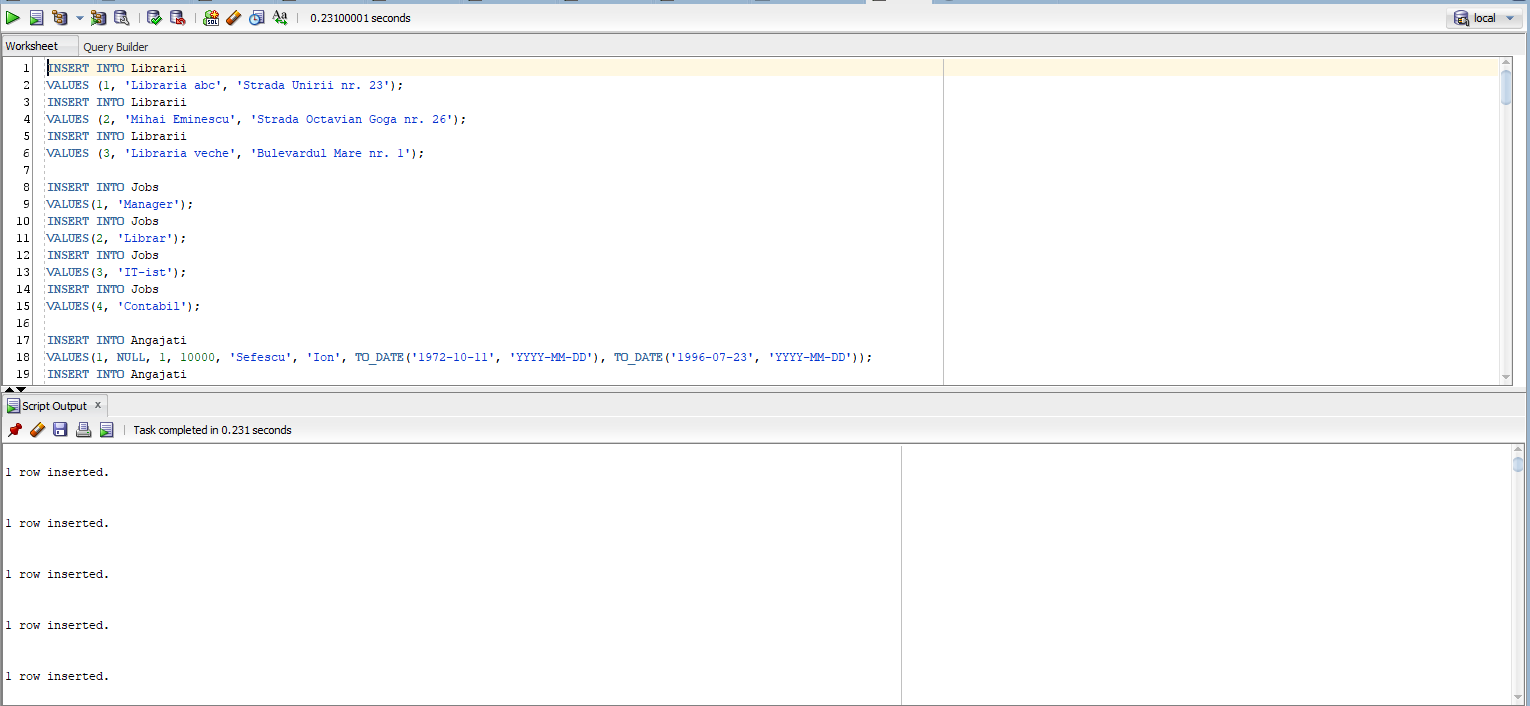
\includegraphics[max width=\linewidth]{imgs/inserts1.png}
\caption{inserts 1}
\label{fig:inserts 1}
\end{figure}
\begin{figure}[!htb]
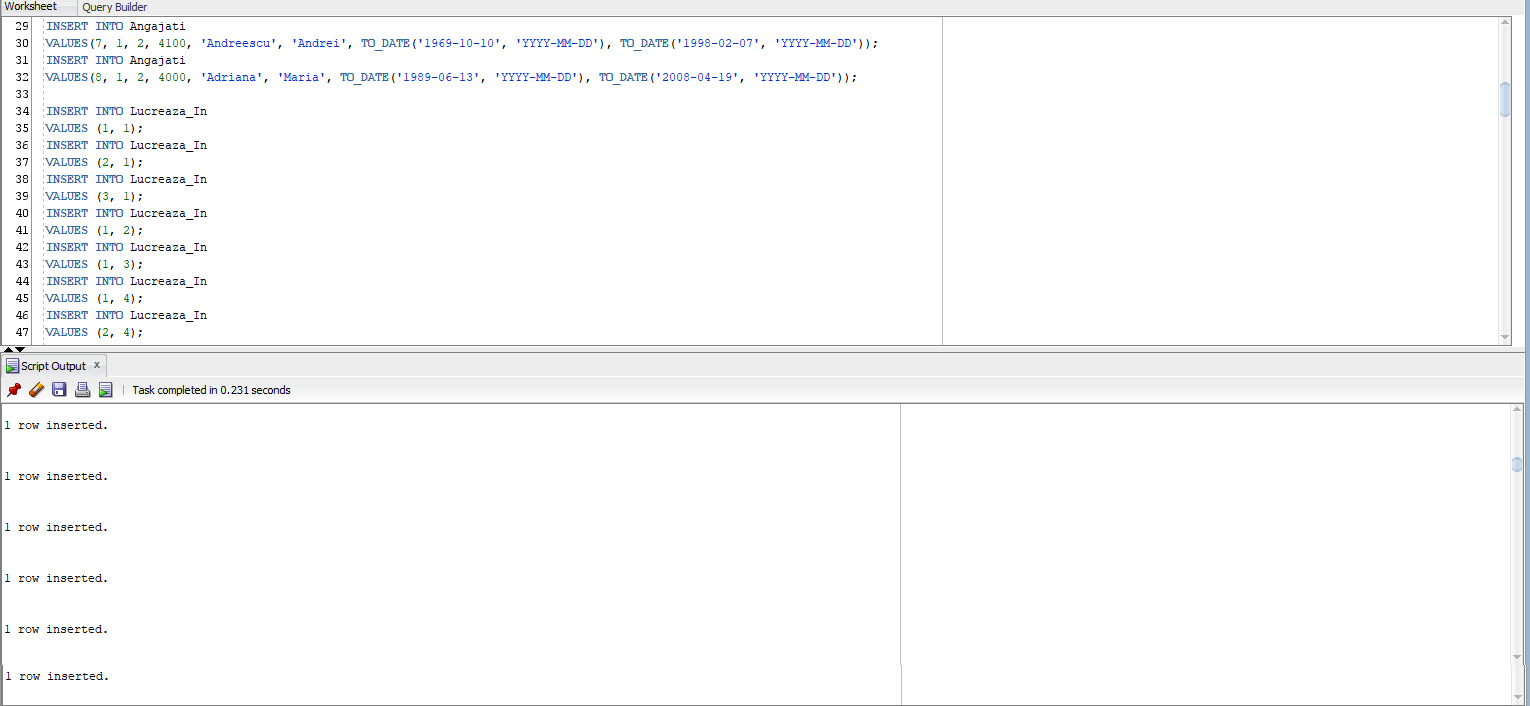
\includegraphics[max width=\linewidth]{imgs/inserts2.png}
\caption{inserts 2}
\label{fig:inserts 2}
\end{figure}
\begin{figure}[!htb]
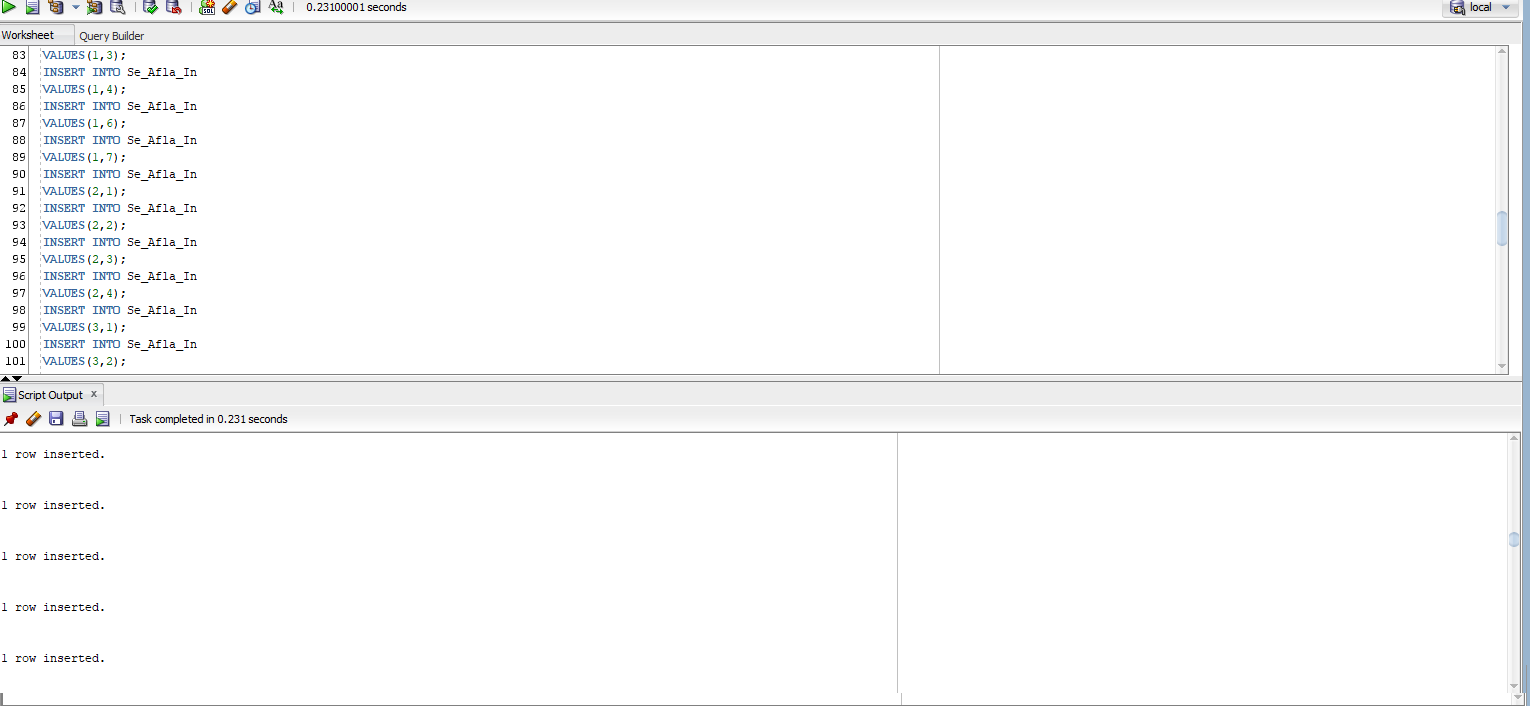
\includegraphics[max width=\linewidth]{imgs/inserts3.png}
\caption{inserts 3}
\label{fig:inserts 3}
\end{figure}
\begin{figure}[!htb]
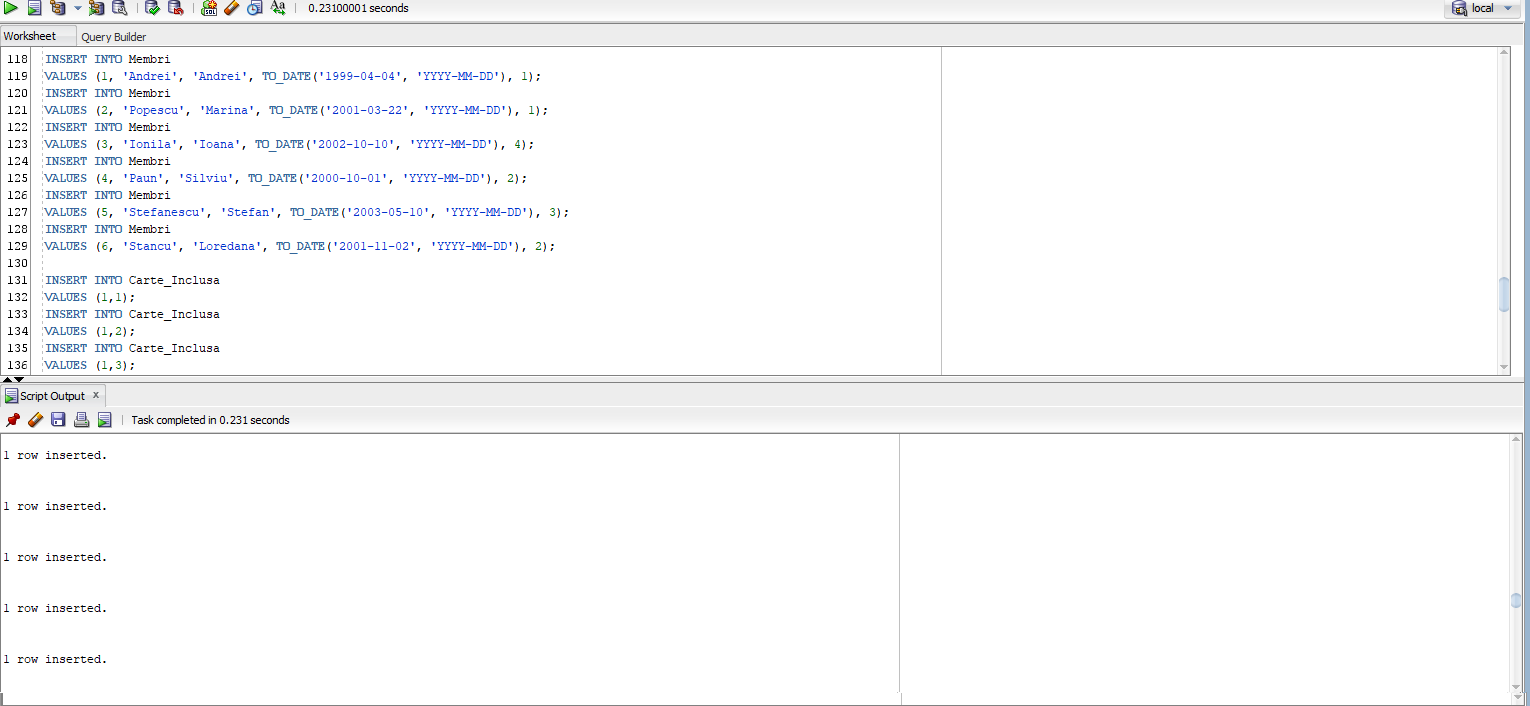
\includegraphics[max width=\linewidth]{imgs/inserts4.png}
\caption{inserts 4}
\label{fig:inserts 4}
\end{figure}
\begin{figure}[!htb]
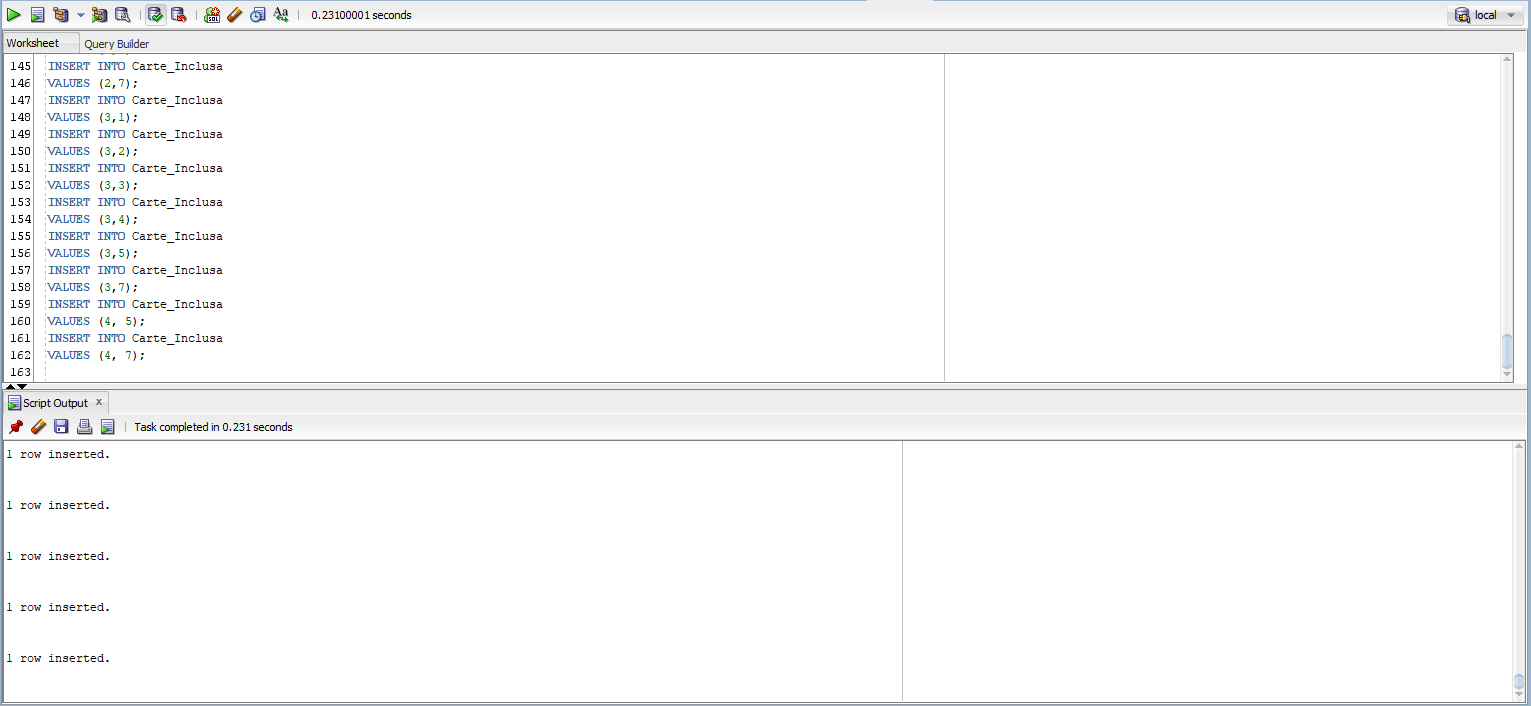
\includegraphics[max width=\linewidth]{imgs/inserts5.png}
\caption{inserts 5}
\label{fig:inserts 5}
\end{figure}
\section{Subprogram cu un tip de colecție studiat}
Am scris un subprogram care determină în care librării se găsește cartea trimisă ca parametru și ce abonamente o includ.\\
\begin{lstlisting}[language=SQL,
	showspaces=false,
	basicstyle=\ttfamily,
	numbers=left,
	numberstyle=\tiny,
	breaklines=true,
	commentstyle=\color{gray}]
-- Un subprogram care determina in care librarii se gaseste cartea introdusa ca parametru si ce abonamente o includ.
CREATE OR REPLACE PROCEDURE ex6 (v_nume_carte carti.denumire%TYPE )IS
TYPE string_tabel IS TABLE OF VARCHAR2(60) INDEX BY PLS_INTEGER;
TYPE number_tabel IS TABLE OF NUMBER INDEX BY PLS_INTEGER;
v_id_carte carti.carte_id%TYPE := NULL;
v_librarii string_tabel;
v_abonamente string_tabel;
v_pret abonamente.plata_lunara%TYPE;
BEGIN
SELECT carte_id INTO v_id_carte
FROM carti
WHERE v_nume_carte = carti.denumire;

SELECT l.denumire BULK COLLECT INTO v_librarii
FROM librarii l, se_afla_in sai
WHERE sai.carte_id = v_id_carte AND sai.librarie_id = l.librarie_id;

DBMS_OUTPUT.put(v_nume_carte || ' se gaseste in librariile: ');
FOR i IN 1..v_librarii.last LOOP
DBMS_OUTPUT.put(v_librarii(i) || ' ');
END LOOP;
DBMS_OUTPUT.NEW_LINE();

SELECT a.abonament_id BULK COLLECT INTO v_abonamente
FROM abonamente a, carte_inclusa ci
WHERE ci.carte_id = v_id_carte AND ci.abonament_id = a.abonament_id;

IF v_abonamente.count = 0 THEN
DBMS_OUTPUT.PUT_LINE('Cartea nu este inclusa in niciun abonament.');
ELSE
DBMS_OUTPUT.PUT(v_nume_carte || ' este inclusa in format digital in abonamentele: ');
FOR i in 1..v_abonamente.last LOOP
SELECT a.plata_lunara INTO v_pret
FROM abonamente a
WHERE a.abonament_id = v_abonamente(i);
DBMS_OUTPUT.PUT('abonamentul ' || v_abonamente(i) || ' cu pretul ' || v_pret || ', ');
END LOOP;
DBMS_OUTPUT.NEW_LINE();
END IF;

EXCEPTION 
WHEN NO_DATA_FOUND THEN
DBMS_OUTPUT.PUT_LINE('Cartea nu exista.');
END;
/
\end{lstlisting}
\begin{figure}[!htb]
	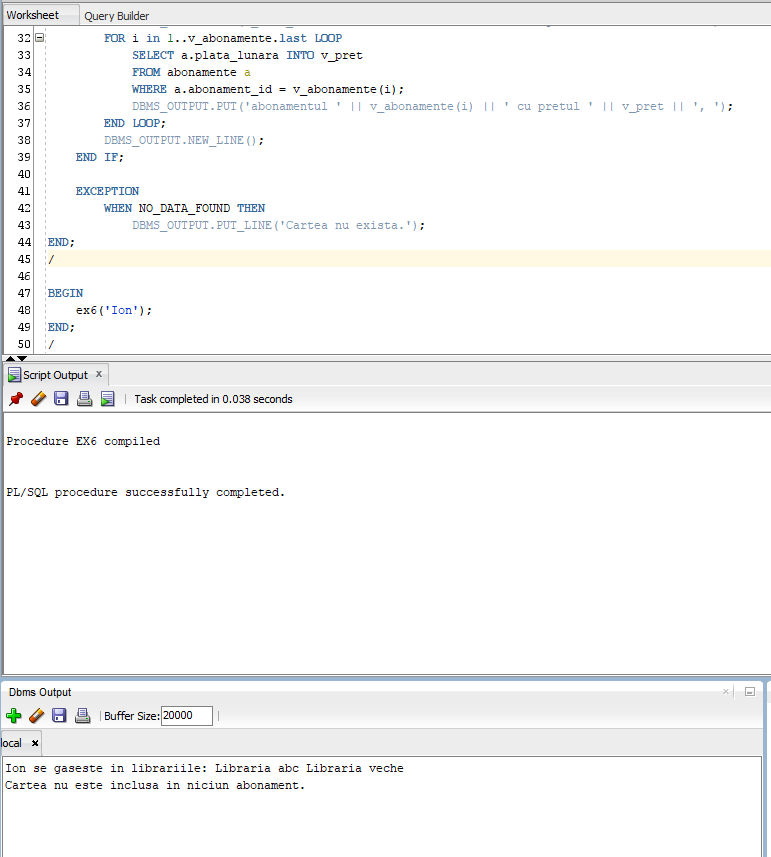
\includegraphics[max width=\linewidth]{imgs/ex6_1.png}
	\caption{Carte care nu exista in vreun abonament}
	\label{fig:ex6_1}
\end{figure}
\begin{figure}[!htb]
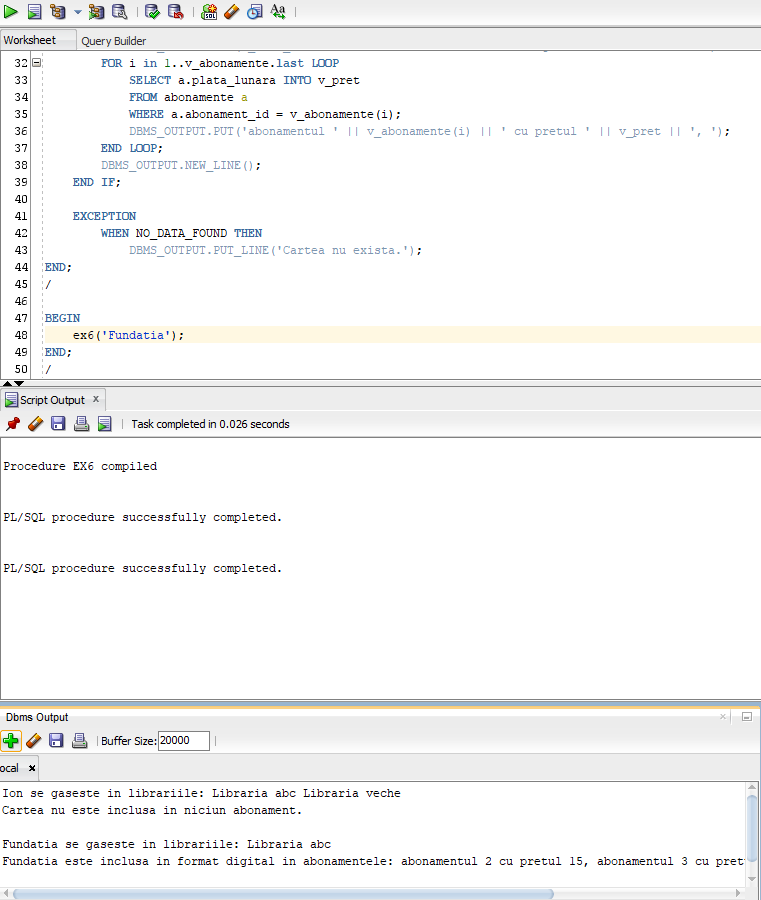
\includegraphics[max width=\linewidth]{imgs/ex6_2.png}
\caption{Carte inclusa in abonamente}
\label{fig:ex6_2}
\end{figure}
\begin{figure}[!htb]
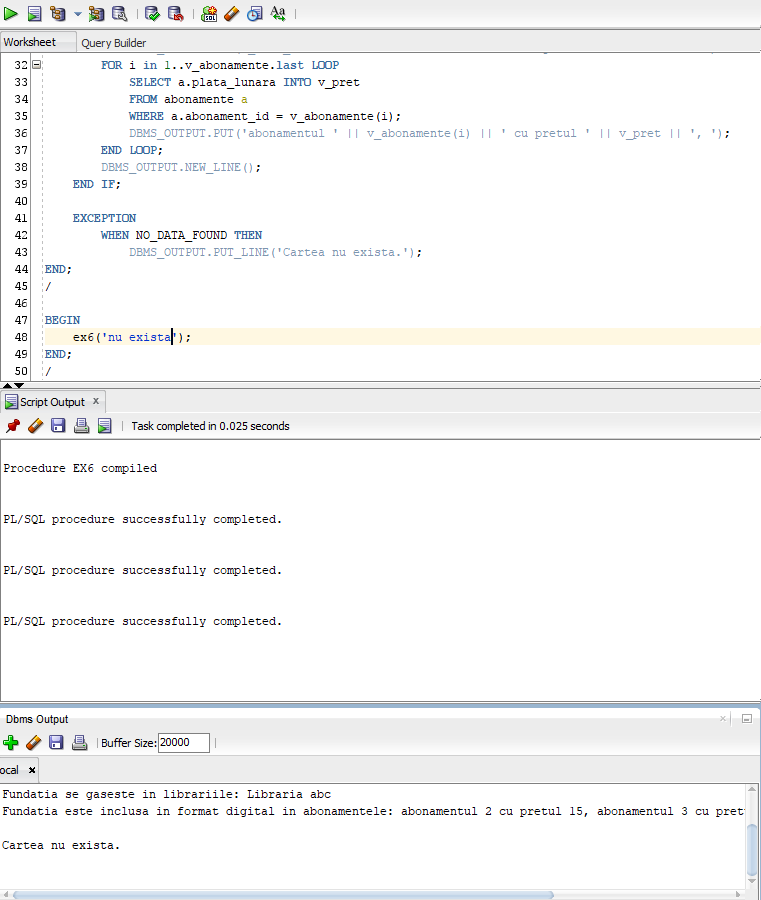
\includegraphics[max width=\linewidth]{imgs/ex6_3.png}
\caption{Carte inexistenta}
\label{fig:ex6_3}
\end{figure}
\section{Subprogram cu un tip de cursor studiat}
Am scris o procedură care caută angajații cu o vechime dată ca parametru cursorului dintr-o librărie dată, de asemenea, ca parametru, și le mărește salariul cu 15%.\\
\begin{lstlisting}[language=SQL,
	showspaces=false,
	basicstyle=\ttfamily,
	numbers=left,
	numberstyle=\tiny,
	breaklines=true,
	commentstyle=\color{gray}]
--O procedura care cauta angajatii cu vechime data ca parametru dintr-o librarie data de asemenea ca parametru si le mareste 
--salariul cu 15%.
CREATE OR REPLACE PROCEDURE ex7 (vechime NUMBER,
cod_librarie librarii.librarie_id%TYPE)
IS
CURSOR c (pvec NUMBER, pcod librarii.librarie_id%TYPE) IS
SELECT a.angajat_id, a.nume, a.prenume, a.manager_id
FROM angajati a, lucreaza_in li
WHERE TRUNC ((SYSDATE) - a.data_angajarii) / 365.5 >= pvec AND li.angajat_id = a.angajat_id AND li.librarie_id = pcod;
BEGIN
FOR i in c(vechime, cod_librarie) LOOP
IF i.manager_id IS NOT NULL THEN
UPDATE angajati
SET salariu = salariu + salariu * 15 / 100
WHERE angajat_id = i.angajat_id;
DBMS_OUTPUT.PUT_LINE('A fost marit salariul anagajtului\ei ' || i.nume || ' ' || i.prenume || ' .');
END IF;
END LOOP;
END;
/
\end{lstlisting}
\begin{figure}[!htb]
	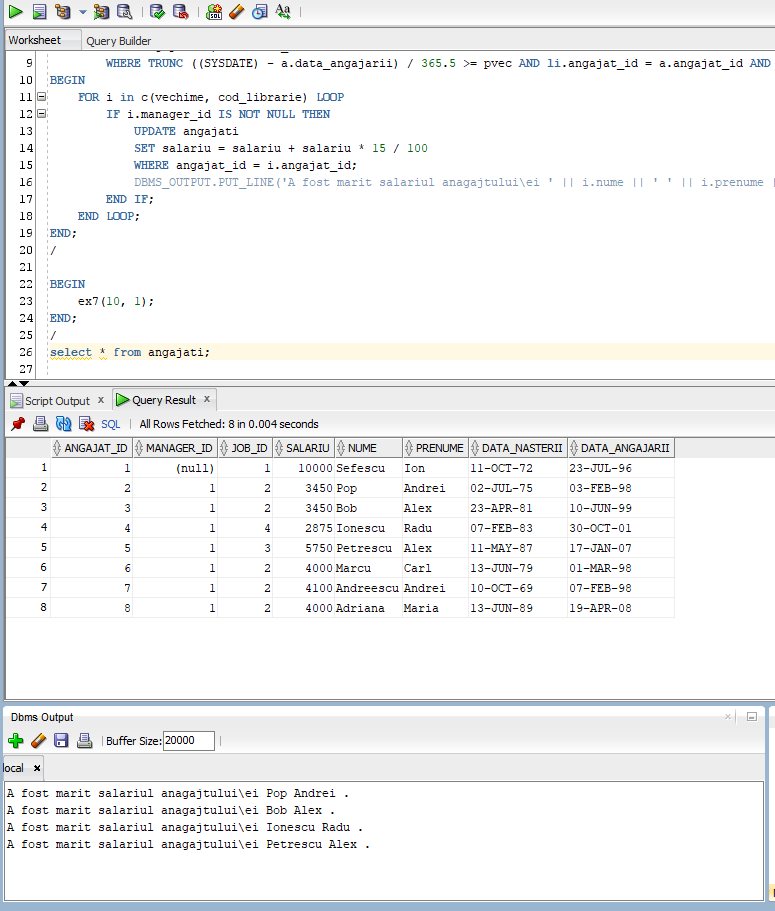
\includegraphics[max width=\linewidth]{imgs/ex7.png}
	\caption{Exemplu de executie + tabel schimbat}
	\label{fig:ex7}
\end{figure}
\section{Subprogram de tip funcție care lucrează cu minim 3 tabele}
Am scris o funcție care, dându-se denumirea unui job, returnează un șir de numere ce reprezintă câți angajați au job-ul respectiv în fiecare librărie.\\
\begin{lstlisting}[language=SQL,
	showspaces=false,
	basicstyle=\ttfamily,
	numbers=left,
	numberstyle=\tiny,
	breaklines=true,
	commentstyle=\color{gray}]
CREATE OR REPLACE TYPE int_table IS VARRAY(3) OF NUMBER;
/
--Dandu-se denumirea unui job, vrem un sir de numere ce reprezinta
--cati angajati au job-ul respectiv in fiecare librarie.
CREATE OR REPLACE FUNCTION f8 (job_name jobs.denumire%TYPE)
RETURN int_table
IS
v_job_id angajati.job_id%TYPE;
v_check NUMBER;
v_old_lib_val NUMBER := -1;
v_counter NUMBER := 1;
v_found_job NUMBER := 0;
retval int_table := int_table(0,0,0);
BEGIN
SELECT job_id INTO v_job_id
FROM jobs
WHERE denumire = job_name;

SELECT COUNT(*) INTO v_check -- verific daca exista angajati cu job-ul dat
FROM angajati a
WHERE a.job_id = v_job_id;
IF v_check = 0 THEN
RAISE_APPLICATION_ERROR(-20000, 'Nu exista angajati cu job-ul dat.');
END IF;

FOR i IN (SELECT l.librarie_id, a.job_id, COUNT(*) c
FROM angajati a, lucreaza_in li, librarii l
WHERE a.angajat_id = li.angajat_id AND li.librarie_id = l.librarie_id
GROUP BY l.librarie_id, a.job_id
ORDER BY l.librarie_id) LOOP
IF v_old_lib_val = -1 THEN -- prima intrare in for
v_old_lib_val := i.librarie_id;
END IF;
IF i.librarie_id != v_old_lib_val THEN -- am ajuns in gruparea pentru urmatoarea librarie
v_counter := v_counter + 1;
v_old_lib_val := i.librarie_id;
IF v_found_job = 0 THEN
retval(v_counter - 1) := 0;
END IF;
v_found_job := 0;
END IF;

IF i.job_id = v_job_id THEN
v_found_job := 1;
retval(v_counter) := i.c;
END IF;
END LOOP;    
RETURN retval;

EXCEPTION
WHEN NO_DATA_FOUND THEN
RAISE_APPLICATION_ERROR(-20000, 'Nu exista jobul dat');
END;
/
\end{lstlisting}
\begin{figure}[!htb]
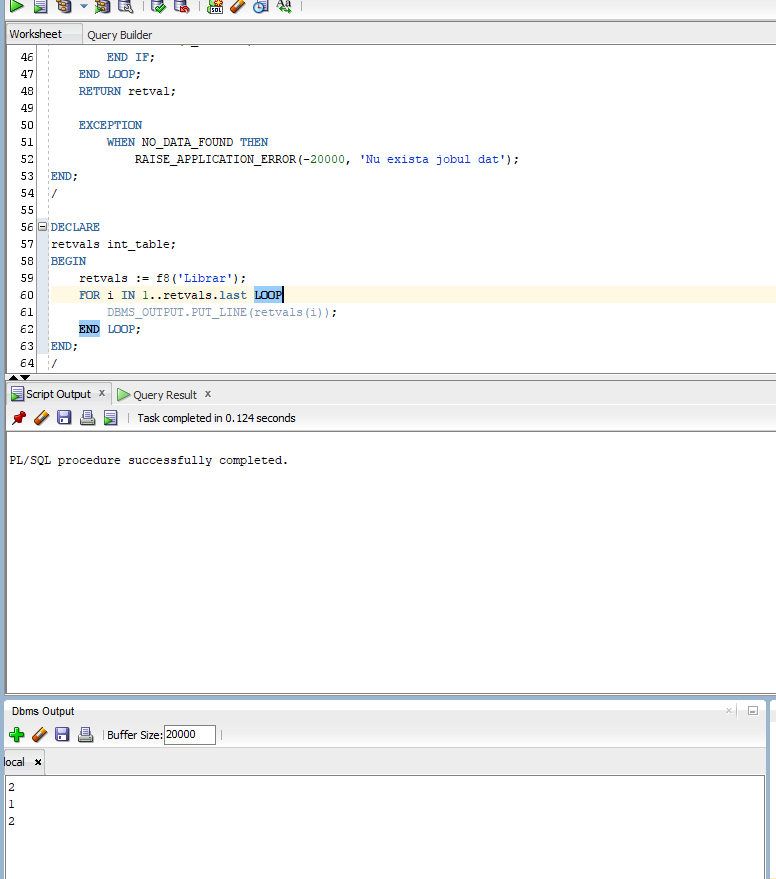
\includegraphics[max width=\linewidth]{imgs/ex8_1.png}
\caption{Fara exceptii}
\label{fig:ex8_1}
\end{figure}
\begin{figure}[!htb]
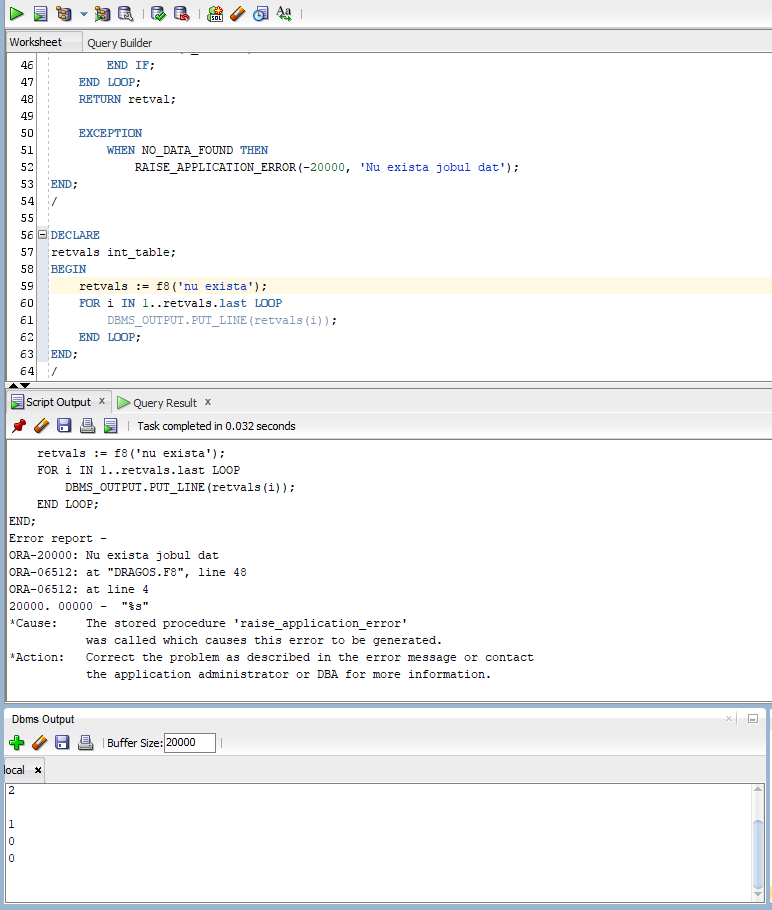
\includegraphics[max width=\linewidth]{imgs/ex8_2.png}
\caption{Job care nu există}
\label{fig:ex8_2}
\end{figure}
\begin{figure}[!htb]
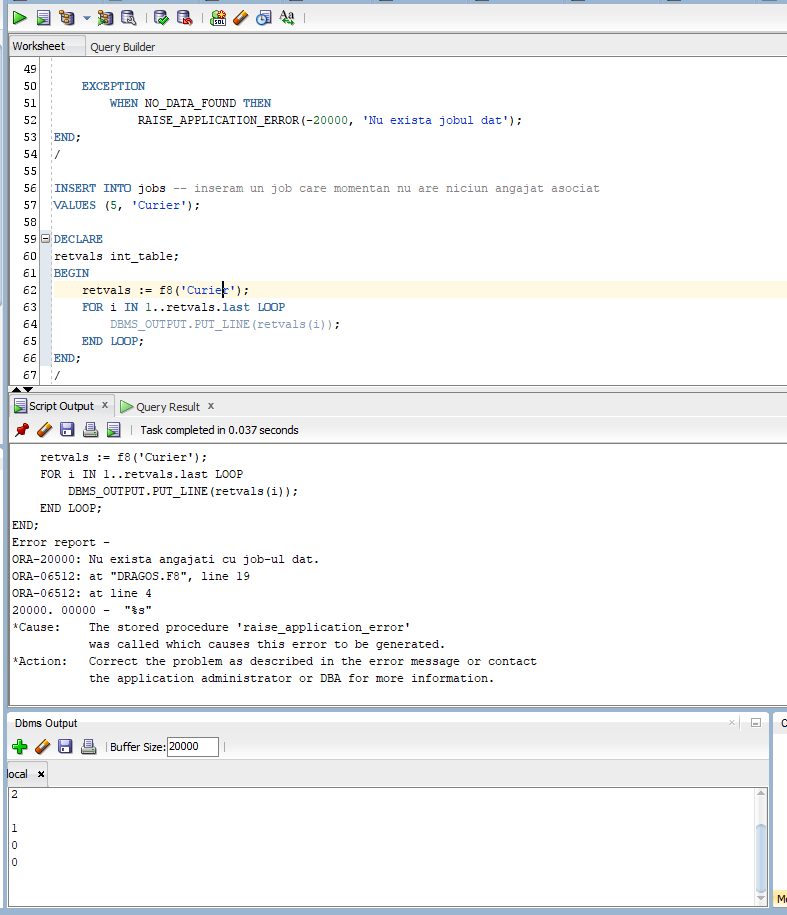
\includegraphics[max width=\linewidth]{imgs/ex8_3.png}
\caption{Nu avem angajați cu job-ul dat}
\label{fig:ex8_3}
\end{figure}
\section{Subprogram de tip procedură care lucrează cu 5 tabele}
Dându-se denumirea unei librării ca parametru, vreau să obțin toți membrii care au abonamente cu cărți din librărie.\\
\begin{lstlisting}[language=SQL,
	showspaces=false,
	basicstyle=\ttfamily,
	numbers=left,
	numberstyle=\tiny,
	breaklines=true,
	commentstyle=\color{gray}]
--Vreau sa obtin o lista cu toti membrii care au abonamente cu carti din libraria data in procedura.
--Lista contine si numele abonamentului despre care este vorba.
CREATE OR REPLACE PROCEDURE p9 (lib_name librarii.denumire%TYPE)
IS
TYPE nume IS RECORD (abonament_id abonamente.abonament_id%TYPE,
nume membri.nume%TYPE,
prenume membri.prenume%TYPE);
TYPE name_table IS TABLE OF nume INDEX BY PLS_INTEGER;
v_lib_id librarii.librarie_id%TYPE;
flag NUMBER := 0;
v_data name_table;
BEGIN
SELECT librarie_id INTO v_lib_id
FROM librarii
WHERE denumire = lib_name;

SELECT a.abonament_id, m.nume, m.prenume BULK COLLECT INTO v_data
FROM membri m, abonamente a, carte_inclusa ci, carti c, se_afla_in sai
WHERE sai.librarie_id = v_lib_id AND sai.carte_id = c.carte_id AND c.carte_id = ci.carte_id AND ci.abonament_id = a.abonament_id AND m.abonament_id = a.abonament_id
GROUP BY a.abonament_id, m.nume, m.prenume;

IF v_data.count = 0 THEN
RAISE_APPLICATION_ERROR(-20000, 'Nu exista membrii cu abonamente care includ carti in libraria ceruta.');
END IF;

FOR i in 1..v_data.last LOOP
DBMS_OUTPUT.PUT_LINE('Abonamentul ' || v_data(i).abonament_id || ', detinut de membrul ' || v_data(i).nume || ' ' || v_data(i).prenume || '.');
END LOOP;

EXCEPTION
WHEN NO_DATA_FOUND THEN
RAISE_APPLICATION_ERROR(-20000, 'Nu exista libraria ceruta.');
END;
/
\end{lstlisting}
\begin{figure}[!htb]
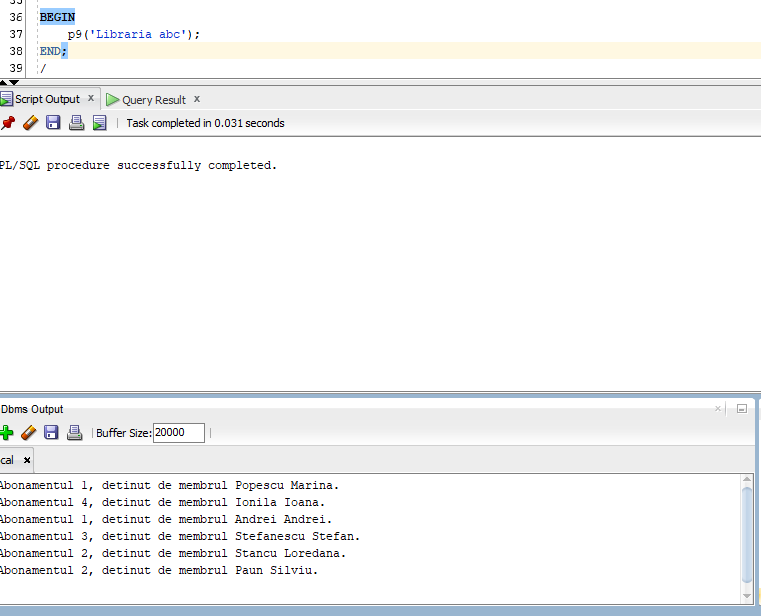
\includegraphics[max width=\linewidth]{imgs/ex9_1.png}
\caption{Fără excepții}
\label{fig:ex9_1}
\end{figure}
\begin{figure}[!htb]
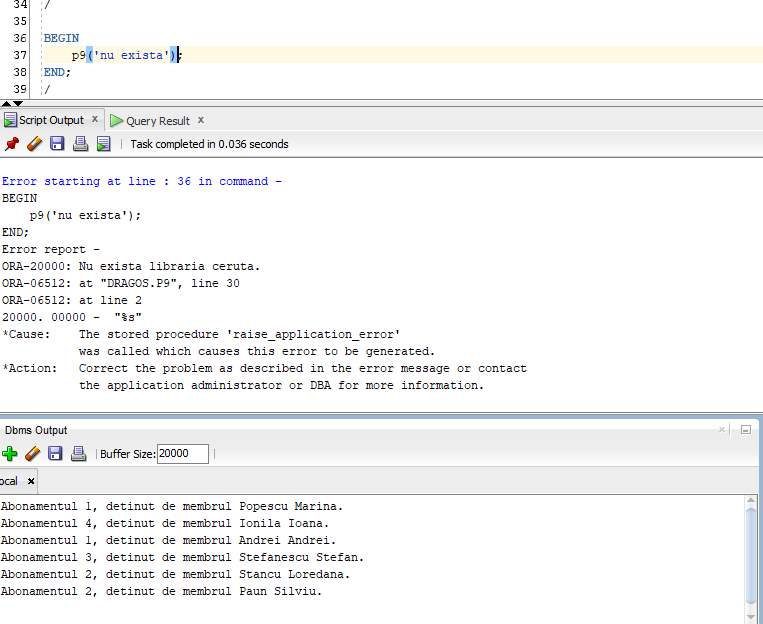
\includegraphics[max width=\linewidth]{imgs/ex9_2.png}
\caption{Librărie care nu există}
\label{fig:ex9_2}
\end{figure}
\begin{figure}[!htb]
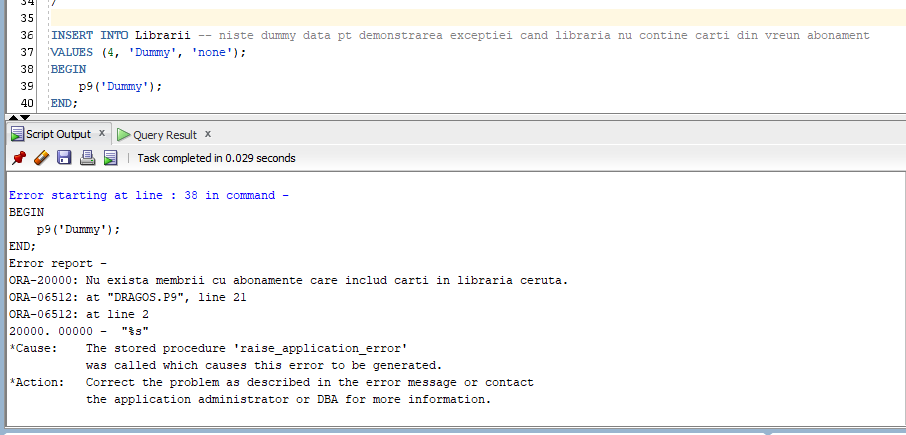
\includegraphics[max width=\linewidth]{imgs/ex9_3.png}
\caption{Librărie care nu conține cărți din vreun abonament}
\label{fig:ex9_3}
\end{figure}
\section{Trigger LMD la nivel de comandă}
Am scris un trigger care interzice schimbarea tabelului Membrii în weekend sau în afara orelor de program ale IT-istului.\\
\begin{lstlisting}[language=SQL,
	showspaces=false,
	basicstyle=\ttfamily,
	numbers=left,
	numberstyle=\tiny,
	breaklines=true,
	commentstyle=\color{gray}]
--Nu e permis sa fie schimbati membrii in timpul weekend-ului sau in afara orelor de program.
CREATE OR REPLACE TRIGGER T10 
BEFORE INSERT OR DELETE OR UPDATE ON Membri
BEGIN
IF (TO_CHAR(SYSDATE, 'D') = 1 OR TO_CHAR(SYSDATE, 'D') = 7)
OR TO_CHAR(SYSDATE, 'HH24') NOT BETWEEN 8 AND 21 THEN
RAISE_APPLICATION_ERROR(-20001, 'Nu se pot face modificari la tabelul membrilor in acest interval orar');
END IF;
END;
/
\end{lstlisting}
\begin{figure}[!htb]
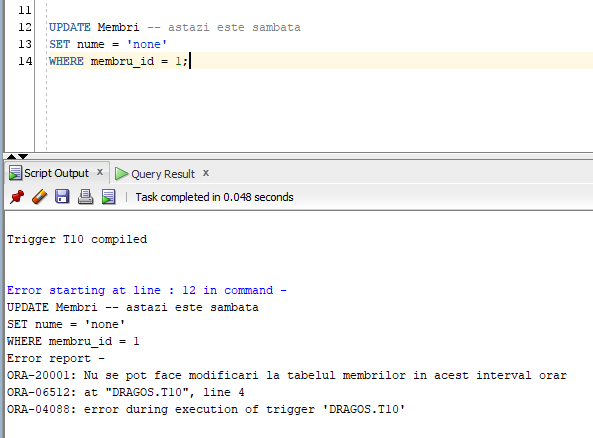
\includegraphics[max width=\linewidth]{imgs/ex10.png}
\caption{Încercare de update sâmbăta}
\label{fig:ex10}
\end{figure}
\section{Trigger LMD la nivel de linie}
Am scris un trigger care, atunci când prețul unei cărți este schimbat, va reflecta schimbarea în prețul abonamentelor ce includ cartea. Deoarece abonamentele sunt deja destul de ieftine, schimbarea va fi efectuată doar când prețul unei cărți este mărit sau când, din păcate, este scoasă din stocul afacerii.\\
Deoarece un astfel de trigger ar solicita un select pe tabelul Cărți, pentru a calcula cât reprezintă ca procentaj din valoarea unui abonament o anumită carte, am avea de a face cu un trigger pe tabele mutating. Pentru a evita eroarea, am folosit un package în care, folosind un trigger LMD la nivel de comandă, voi stoca tabelul Cărți într-o colecție. Deși nu este necesar, am stocat și tabelul Abonamente, pentru a mai simplifica din codul trigger-ului la nivel de linie.\\
\begin{lstlisting}[language=SQL,
	showspaces=false,
	basicstyle=\ttfamily,
	numbers=left,
	numberstyle=\tiny,
	breaklines=true,
	commentstyle=\color{gray}]
--Cand pretul unei carti este schimbat, vrem ca schimbarea sa fie reflectata si in abonament, in cazul in care scumpim cartea
--Daca scoatem o carte din stoc, vom ieftini abonamentul cu procentajul pe care pretul cartii il reprezenta din intregul pachet al abonamentului.
--Pt a evita trigger mutating, vom folosi o colectie intr-un pachet, care este intializata cu un trigger la nivel de comanda.
CREATE OR REPLACE PACKAGE trig_help 
AS
TYPE abo IS TABLE OF abonamente%ROWTYPE INDEX BY PLS_INTEGER;
TYPE car IS TABLE OF carti%ROWTYPE INDEX BY PLS_INTEGER;
TYPE ci  IS TABLE OF carte_inclusa%ROWTYPE INDEX BY PLS_INTEGER;
abonamente_c abo;
carte_c car;
carte_inclusa_c ci;
end;
/
CREATE OR REPLACE TRIGGER T11_HELP
BEFORE UPDATE OR DELETE ON carti
BEGIN
SELECT * BULK COLLECT INTO trig_help.abonamente_c
FROM abonamente;
SELECT * BULK COLLECT INTO trig_help.carte_c
FROM carti;
SELECT * BULK COLLECT INTO trig_help.carte_inclusa_c
FROM carte_inclusa;
END;
/

CREATE OR REPLACE TRIGGER T11
BEFORE UPDATE OR DELETE ON carti
FOR EACH ROW
DECLARE 
buffr number;
v_pret_total NUMBER(4);
v_pret_carte NUMBER(4);
v_crestere_prop NUMBER(4);
BEGIN
IF UPDATING THEN
IF :NEW.carte_id != :OLD.carte_id THEN
RAISE_APPLICATION_ERROR(-20001,'Nu este permisa schimbarea cheiilor primare din tabelul Carte');
END IF;

FOR i in 1..trig_help.abonamente_c.last LOOP
v_pret_total := 0;
IF :NEW.pret > :OLD.pret THEN -- ne intereseaza sa modificam doar daca pretul cartii e crescut
FOR j in 1..trig_help.carte_c.last LOOP
buffr := 0;
SELECT COUNT(*) INTO buffr --nu o sa avem mutating, pt ca id-ul cartii nu se schimba
FROM carte_inclusa ci
WHERE ci.abonament_id = trig_help.abonamente_c(i).abonament_id AND ci.carte_id = trig_help.carte_c(j).carte_id;

IF buffr > 0 THEN
v_pret_total := v_pret_total + trig_help.carte_c(j).pret; -- deoarece valorile sunt luate cu un trigger before, e ca si cum am apela :OLD pt valoarea schimbata
END IF;
END LOOP;

v_crestere_prop := :NEW.pret / :OLD.pret;

UPDATE abonamente -- crestem proportia
SET plata_lunara = plata_lunara + (:NEW.pret / v_pret_total) * plata_lunara
WHERE abonament_id = trig_help.abonamente_c(i).abonament_id;
END IF;
END LOOP;
ELSE --DELETING
FOR i in 1..trig_help.abonamente_c.last LOOP
v_pret_total := 0;
FOR j in 1..trig_help.carte_c.last LOOP
buffr := 0;
-- trebuie sa folosim colectia din pachet, deoarece id-ul cartii este scos si din carte_inclusa
FOR k in 1..trig_help.carte_inclusa_c.last LOOP
IF trig_help.carte_inclusa_c(k).abonament_id = trig_help.abonamente_c(i).abonament_id
AND trig_help.carte_inclusa_c(k).carte_id = trig_help.carte_c(j).carte_id THEN
buffr := 1;
END IF;
END LOOP;

IF buffr > 0 THEN
v_pret_total := v_pret_total + trig_help.carte_c(j).pret; -- deoarece valorile sunt luate cu un trigger before, e ca si cum am apela :OLD pt valoarea schimbata
END IF;
END LOOP;

UPDATE abonamente -- crestem proportia
SET plata_lunara = plata_lunara - (:OLD.pret / v_pret_total) * plata_lunara
WHERE abonament_id = trig_help.abonamente_c(i).abonament_id;
END LOOP;
END IF;
END;
/
\end{lstlisting}	
\begin{figure}[!htb]
	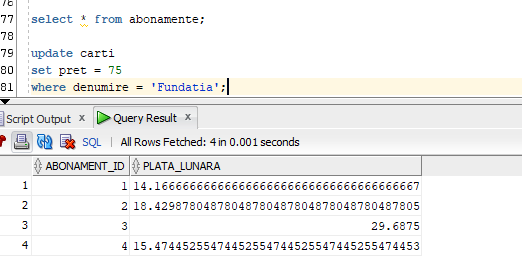
\includegraphics[max width=\linewidth]{imgs/ex11_1.png}
	\caption{Update-ul se reflectă în prețurile abonamentelor}
	\label{fig:ex11_1}
\end{figure}
\begin{figure}[!htb]
	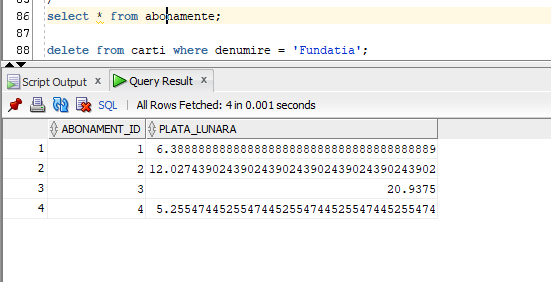
\includegraphics[max width=\linewidth]{imgs/ex11_2.png}
	\caption{Delete}
	\label{fig:ex11_2}
\end{figure}
\section{Triger LDD}
Pentru trigger-ul LDD, am implementat un tabel de tip audit.\\
\begin{lstlisting}[language=SQL,
	showspaces=false,
	basicstyle=\ttfamily,
	numbers=left,
	numberstyle=\tiny,
	breaklines=true,
	commentstyle=\color{gray}]
--Voi face un audit, pentru a avea un istoric al comenzilor facute pe baza de date.
CREATE TABLE audit_lib
(utilizator VARCHAR2(50),
nume_bd VARCHAR2(50),
eveniment VARCHAR2(50),
nume_obiect VARCHAR2(50),
data DATE);

CREATE OR REPLACE TRIGGER T12
AFTER CREATE OR DROP OR ALTER ON SCHEMA
BEGIN
INSERT INTO audit_lib
VALUES (SYS.LOGIN_USER, SYS.DATABASE_NAME, SYS.SYSEVENT,
SYS.DICTIONARY_OBJ_NAME, SYSDATE);
END;
/
\end{lstlisting}	
\begin{figure}[!htb]
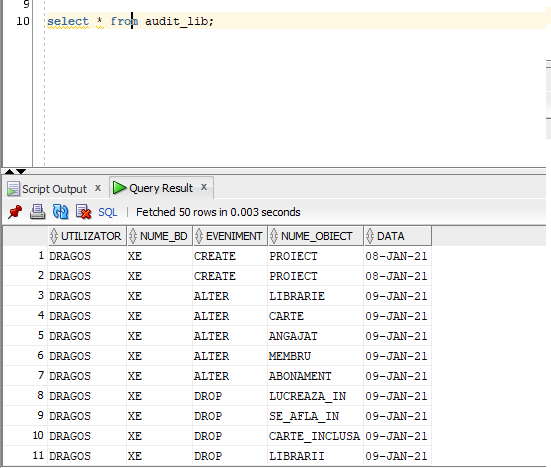
\includegraphics[max width=\linewidth]{imgs/ex12.png}
\caption{Tabelul audit a fost creat inaintea restului de tabele}
\label{fig:ex12}
\end{figure}
\end{document}